\subsection{Architektur eines \ac{DBMS}}



\begin{figure}[h]
  \centering
  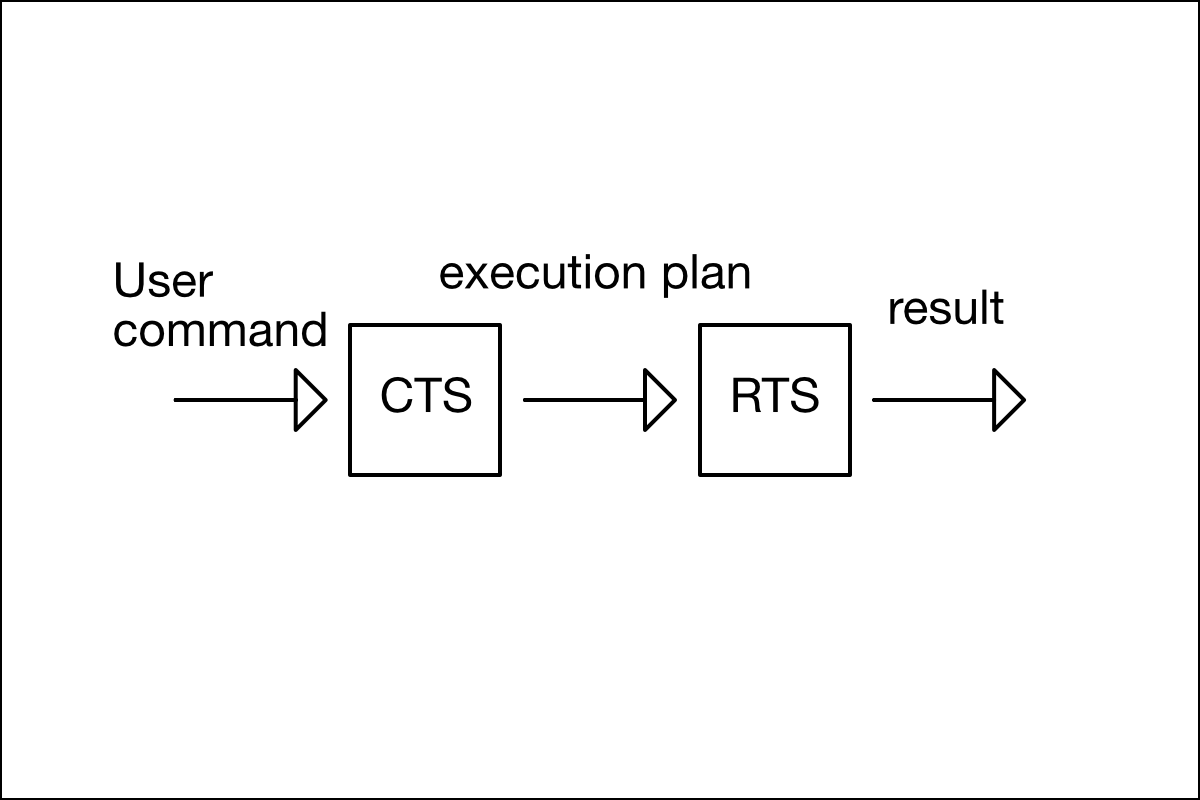
\includegraphics[width=\textwidth]{02_Grundlagen/DBMS_Architecture.png}
  \caption{\ac{DBMS} Architektur}
  \label{SearchSpace}
\end{figure}


Ein \ac{DBMS} lässt sich grob in zwei Teile gliedern: \ac{CTS} und \ac{RTS}. Jedes Teilsystem verfolgt eine eigene Aufgabe. Eine Kommunikation zwischen den Systemen findet immer unidirektional statt. Das System startet mit einem Nutzerkommando. Es wird in das \ac{CTS} eingegeben und von ihm in eine für das \ac{CTS} bearbeitbare Form gebracht, die dann durch das \ac{RTS} ausgeführt werden kann. Das Resultat dieses Prozesses wird an den User als Ergebnis zurückgeliefert.

Die Nutzerkommandos können variieren. Neben Anfragen (Queries) können auch Indexe erstellt, Schemaveränderungen vorgenommen und Datensätze verändert werden, um nur einige mögliche Kommandos zu nennen. Im Folgenden wird sich auf die Anfrage konzentriert.

Vor der Verarbeitung einer Anfrage muss die Anfrage formuliert werden. Dies geschieht bei relationalen Datenbanksystemen i.d.R. in \ac{SQL}. \ac{SQL} ist eine deklarative Anfragesprache, die sich als Standard in diesem Bereich durchgesetzt hat. Die fertige Anfrage bildet den Input, der in das Datenbanksystem übergeben wird und zuerst im \ac{CTS} ankommt. Dort kann die Anfrage entweder durch einen \ac{QC} oder durch einen \ac{QI} verarbeitet werden.

Der erste Schritt, der innerhalb des \ac{CTS} vorgenommen wird, ist die Umwandlung der Anfrage in eine interne Repräsentationsform. Beispielsweise muss eine Anfrage die in \ac{SQL} formuliert ist und als String vorliegt mit einem Parser verarbeitet werden. Diese Umwandung geschieht bei einem \ac{QI} (vgl. Abb. \ref{DBMS_Interpreter})  im selben Schritt, in dem auch Rewriter zum Einsatz kommen können. Bei Rewritern handelt es sich um Funktionen, die die Anfrage umformulieren. Für \ac{QI} ist es nicht notwendig, dass ein Rewriter zum Einsatz kommt. Das Ergebnis dient in jedem Falle als Input für das \ac{RTS}.


\begin{figure}[h]
  \centering
  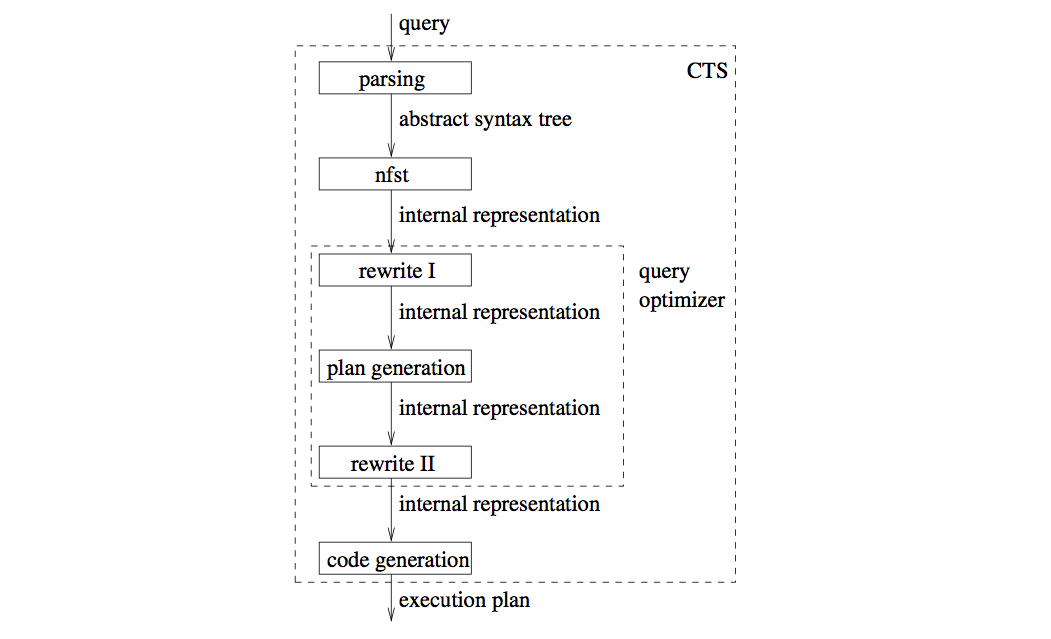
\includegraphics[width=\textwidth]{02_Grundlagen/QC_Architecture.png}
  \caption{\ac{QC} Architektur}
  \label{QC_Architecture}
\end{figure}

Im Gegensatz zum \ac{QI} sind bei einem \ac{QC} mehr Schritte involviert und die Architektur des \ac{QC} (vgl. Abb. \ref{QC_Architecture}) ist daher unterschiedlich. Am Beginn steht der Query Parser. Er wandelt die Anfrage, beispielsweise einen String, in einen internen, abstrakten Syntax baum um. Dier Baum wird durch ein nfst in eine Interne repräsentation gebracht. Die so formatierte Query ist der Input des \ac{QO}. Das Ergebnis wird mit einem Code Generator in einen ausführbaren Plan umgewandelt und dann an das \ac{RTS} weitergeleitet.

Der \ac{QO} selbst führt zu Beginn einen Rewrite durch. Ein Plangenerator kommt zum Einsatz und findet den optimalen Plan. Daraufhin wird mit einem weiteren Rewriter die Anfrage weiterverarbeitet und an den \ac{QC} zurückgegeben.
